\section{Anvendelse af elliptiske kurver i kryptologi}
At bruge tal- og gruppeteori til forskellige krypteringsalgoritmer, er et af de mest populære konkrete eksempler på hvordan denne type af matematik kan bruges. Det er også en af de vigtigste emner indenfor matematik i nyere tid, da det ligger til grund for alt digitalt lige fra banker til hjemmesider. Med punkter på elliptiske kurver, kan vi altså sikre det meste af internettet fra tredjemænd i at kunne kigge med!

\subsection{Assymetrisk kryptering}
Assymetrisk- eller public-key kryptering betegner et system hvor alle parter har en offentlig- og en privat nøgle (\cite{seanriley2017}). Den offentlige nøgle, må alle parter i systemet kende til, mens den private nøgle holdes hemmelig. For overskuelighedens skyld kalder vi de to parter i systemet for Alice og Bob.

I et assymetrisk kryptosystem kan Bob og Alice sende krypterede beskeder til hinanden ved brug af hinandens offentlige nøgler uden at en tredjepart kan læse dem. Den eneste måde for en tredjepart at læse deres beskeder vil være ved at finde ud af hvad deres private nøgler er. Der findes mange forskellige algoritmer til assymetrisk kryptering. Jeg har dog valgt at kigge nærmere på \code{Elliptic-Curve Diffie-Hellman key exchange}. 

\subsubsection{Public-Key Exchange - ECDH}
Elliptic-Curve Diffie-Hellman key exchange er en måde til at kombinere Alice og Bob’s public keys sammen således at man får en ny nøgle der kan udføres symmetrisk kryptering med. test

\begin{figure}[htbp]
\centering
\begin{subfigure}{.5\textwidth}
  \centering
  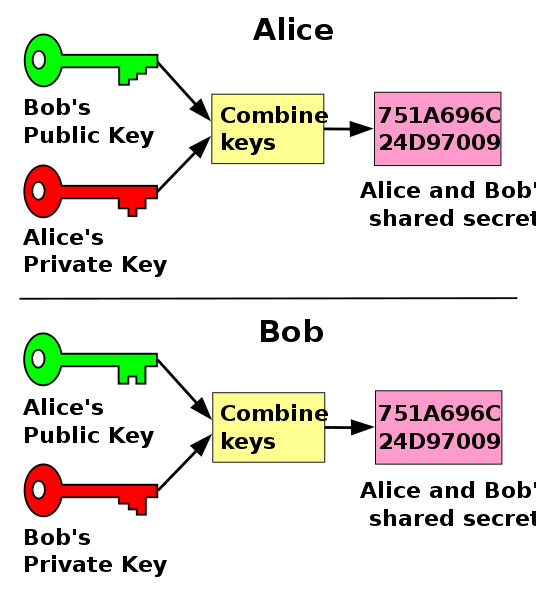
\includegraphics[width=0.9\linewidth]{images/Public_key_shared_secret.svg.png}
  \caption{(\cite{gothberg_2006})}
  \label{fig:sub1}
\end{subfigure}%
\begin{subfigure}{.5\textwidth}
  \centering
  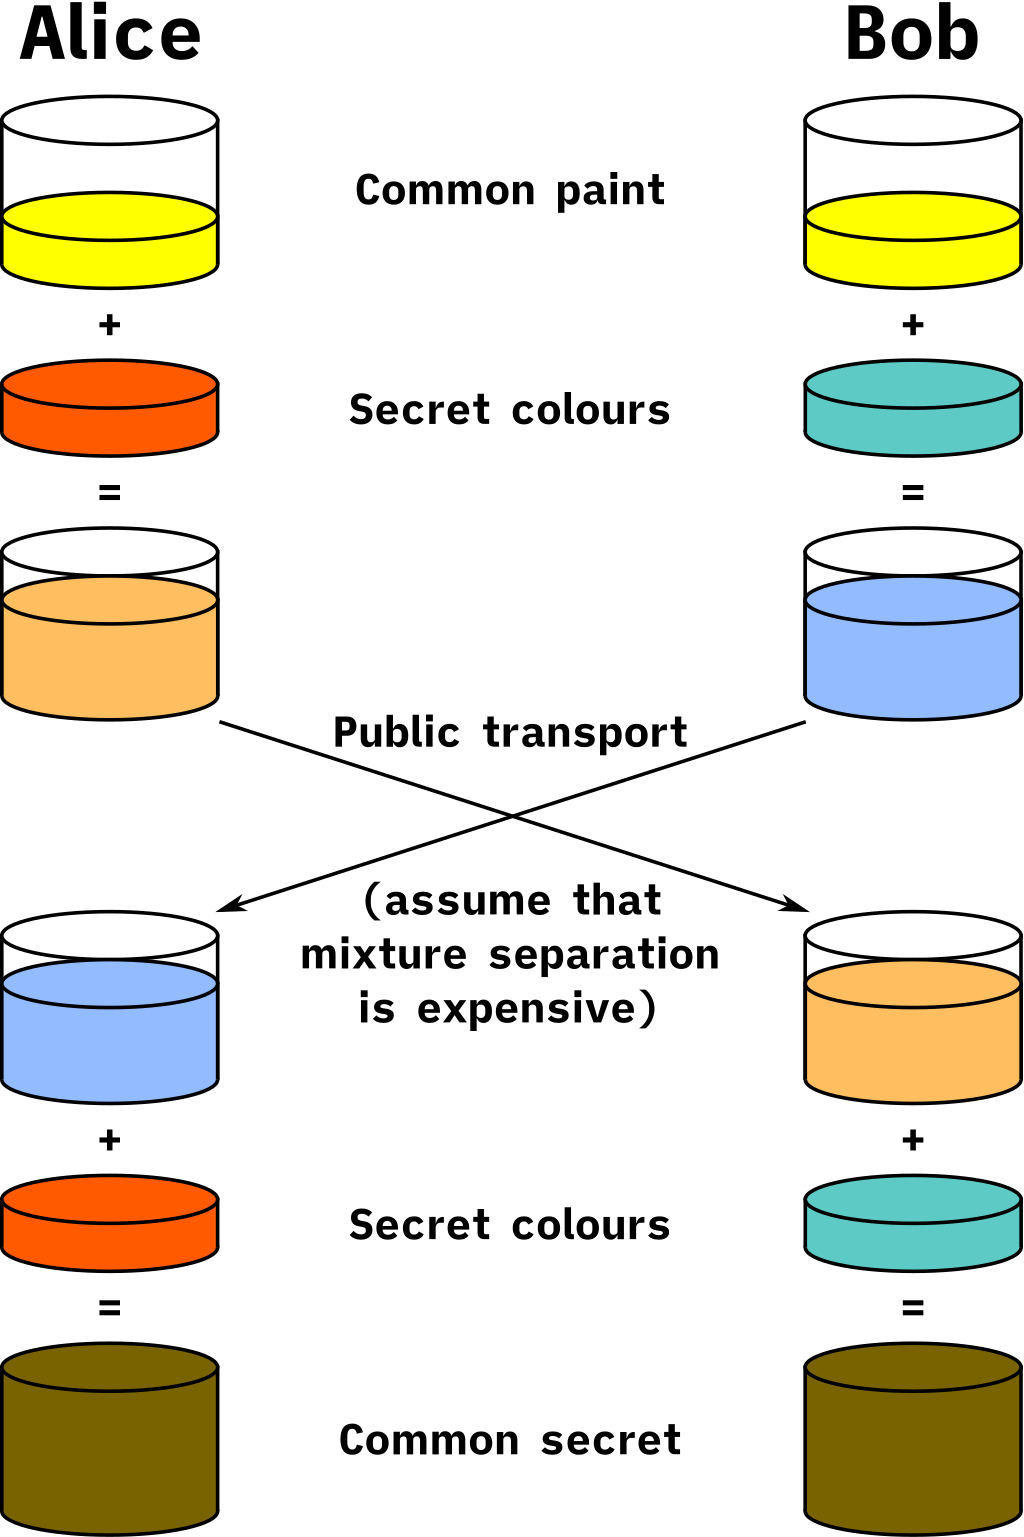
\includegraphics[width=0.7\linewidth]{images/1024px-Diffie-Hellman_Key_Exchange.svg.png}
  \caption{(\cite{Avinck_2011})}
  \label{fig:sub2}
\end{subfigure}
\caption{Illustration af Diffie-Hellmann key Exchange}
\end{figure}

På overstående figurer ses to forskellige måder til at vise hvordan et Diffie-Helmann key exchange hænger sammen. Vi kigger først på figuren til højre. Alices private nøgle vil være den mørkeorange, mens hendes offentlige nøgle er den lyse orange. Hun sender nu sin lyse orange farve til Bob som kombinerer den med sin private nøgle og får: \code{(orange+gul)+turkis=fælles hemmelighed}. Det samme kan Alice gøre: \code{(turkis+gul)+orange=fælles hemmelighed}. Vi får den samme hemmelighed, da operationen er associativ. Hermed er der udført et key-exchange som parterne hver især nu kan bruge til symmetrisk kryptering og sende beskeder til hinanden. Dette kunne eksempelvis gøres med AES-kryptering. Vi kigger nu mere teknisk på hvordan det fungerer i forbindelse med elliptiske kurver \code{ECDH}.
\begin{table}[h]
\label{tab:key_exchange}
\begin{tabular}{|l|l|l|}
\hline
\textbf{Alice}                                                                                                                                                          & \textbf{Public Space}                                                                                                                                                  & \textbf{Bob}                                                                                                                                                       \\ \hline \hline
\begin{tabular}[c]{@{}l@{}}Alice vælger sin private nøgle \\ ved at tage et tilfældigt heltal \\ mellem $1 \leq \alpha \leq n-1$. \\ Privatnøgle $=\alpha$\end{tabular} & \begin{tabular}[c]{@{}l@{}}$p$ primtal\\ $A, B$ koefficienter til den\\ elliptiske kurve\\ $G$ generatorpunktet\\ $n$ ordenen (antal punkter i\\ legemet)\end{tabular} & \begin{tabular}[c]{@{}l@{}}Bob vælger sin private nøgle\\ ved at tage et tilfældigt heltal \\ mellem $1 \leq \alpha \leq n-1$.\\ Privatnøgle $=\beta$\end{tabular} \\ \hline
\begin{tabular}[c]{@{}l@{}}Udregner nyt punkt ved \\ skalarmultiplikation:\\ $$ A = \alpha \cdot G$$\end{tabular}                                              &                                                                                                                                                                        & \begin{tabular}[c]{@{}l@{}}Udregner nyt punkt ved \\ skalarmultiplikation:\\ $$ B = \beta \cdot G$$\end{tabular}                                          \\ \hline
Modtager $B=(x_B, y_B)$                                                                                                                                                  & \begin{tabular}[c]{@{}l@{}}$A=\alpha \cdot G = (x_A, y_A)$\\ $B = \beta \cdot G = (x_B, y_B)$\end{tabular}                                                                         & Modtager $A=(x_A, y_A)$                                                                                                                                             \\ \hline
\begin{tabular}[c]{@{}l@{}}Udregner nyt punkt ved\\ skalarmultiplikation:\\ $P=\alpha \cdot B= \alpha \cdot (\beta \cdot G)$\end{tabular}                                                   &                                                                                                                                                                        & \begin{tabular}[c]{@{}l@{}}Udregner nyt punkt ved\\ skalarmultiplikation:\\ $P=\beta \cdot A = \beta \cdot (\alpha \cdot G)$\end{tabular}                                              \\ \hline
\end{tabular}
\caption{Gennemgang af ECDH: Elliptic Curve Diffie-Helmann key-exchange}
\label{tab:key_exchange_diffie}
\end{table}
\FloatBarrier
Hermed har Alice og Bob fået en fælles nøgle, som de kan bruge til at kryptere beskeder med. 
Bemærk at hvis MITM \textit{(man in the middle)} skal kunne finde frem til $P$ kræver det at de enten kender $\alpha$ eller $\beta$. Umiddelbart kunne det tænkes, at man kan løse udtrykket $\alpha = \frac{A}{G}$, men da $G$ er et element kan vi ikke dividere på denne måde, da division bliver til det inverse element og hermed et helt andet punkt. 
